\section{Methodology}
\label{sec:background}
To address complexity of macroeconomic predictions, this research implements a environment, which prioritizes reproducibility, data realism, model understanding. The following hypotheses are formulated research approach:

\textbf{Hypothesis 1: Lag-aware data improves accuracy of forecasting comparing to the raw naive data} Research will test this experimenting with the raw model inputs predictions and lag aware. 

\textbf{Hypothesis 2: Combination of lstm model with xgboost model provide additional insights about the field and macroeconomics indicators prediction} Research trains both models and compares them.

\textbf{Hypothesis 3: Model explainability helps improve models and address weak points} Research executes explainability reports on models and tries to make sure that all important features are used by the model, depending on the result model must be improved.

In order to prove these hypotheses, research will describe progress of project from the beginning to the final model inference.

\subsection{Dataset Collection}
\label{sec:data_collection}
Starting from the beginning custom dataset collection was selected over already existed datasets on the internet network, the main reason behind this decision is aim to train model german economy specific. The reasons behind that decision is because models like \textbf{LSTM} or \textbf{XGBoost} would struggle to grasp different countries economic differences, thus lowering accuracy of model and making weight updates more chaotic. Model trained on mixed dataset might struggle with finding relationship between features and examples where certain learned correlation doesn't apply might poison model. One feature in one country might be really viable, while for the others it is not so relevant and thus it will also harm xai purpose in this research. 

\subsection{Data sources}

\subsubsection{FRED Economic Data (Federal Reserve Bank of St. Louis)}
\textbf{Scope}: Over 800,000 economic datasets, describing 100+ contries \\
\textbf{Advantages}: Convenient API for programmatic access \\
\textbf{Relevant Series}: Available many macroeconomic data (GDP, unemployment, inflation, interest rates) \\

\subsubsection{World Bank Open Data}
\textbf{Scope}: Macroeconomic indicators for more than 200 contries\\
\textbf{Advantages}: Bigger dataset all around the the world\\
\textbf{Relevant Series}: Almost the same indicators as FRED\\

While considering both options for data source \textit{FRED} had more indicators which was applicable to germany and \textit{World Bank Open Data} was missing several indicators.


The following indicators are core, they where selected as the most viable for the forecasting and classification, applying diverse pressure from different sides of the economy: \\
\indent \textbf{German GDP}: One of the most major economical indicators, which has the most correlation for the goals of predicting next quarter GDP and also classifying economical cycles. GDP represents all the items produced in country and thus might be metric of country success and many macroeconomic metrics which is being predicted using machine learning will be dependent on GDP.  \\
\indent \textbf{German Unemployment Rate}: This economical indicator is used in dataset, because it shows how fully is used contries labor and how much money country has to spend on payouts. When this indicator has extreme high values it might be a sign of a \textit{recession}. \\
\indent \textbf{German Inflation (CPI)}: Indicates how stable price on items currently in country. Extreme values of this indicator might be signaling overworked economy, which is might turn into recession state. This indicator is interesting in particulary for XGBoost model classification.

Many other has been selected and listed here in order of importance: \textit{Economic Policy Uncertainty (EPU) Index}, \textit{ECB Interest Rate}, \textit{German Manufacturing PMI}, \textit{Ifo Business Expectations}, \textit{Industrial Production}, \textit{Exports of Goods}, \textit{Factory Orders} ... the rest indicators are available inside of repository dataset.


\subsection{Data Preprocessing}
\label{sec:data_preprocessing}


\subsubsection{Dataset procession}

\textbf{Input Dataset} \\
- \textbf{Shape}: 947 rows × 17 columns \\ 
- \textbf{Available data}: 1947 to 2025, with significant amount of nan in early 1940s

\noindent\textbf{Output Dataset} \\
- \textbf{Shape}: 268 rows × 310 columns \\ 
- \textbf{Available data}: 1992 to 2025, clear data \\
- \textbf{Changes}: Processed rows, with expanded features and classification labels for economic cycles

\subsubsection{Lag data creation}
This preprocessing is creates lagged features for indicators example is: \\
GermanGDP, GermanGDPlag1, GermanGDPlag3, GermanGDPlag6, GermanGDPlag12. Each of these lag metric represents lag,  1 month lag represent immediate state of signal one month ago, 3 month lag represent quarterly changes for metrics which are published every quarter like GDP, 6 month lag is used for capturing medium term changes, 12 month lag represent yearly base. Each of 17 indicators required 4 lag features, thus resulting in 68 columns.

\subsubsection{Moving averages creation and standard deviation}
Project uses moving averages and standard deviations for smoothing each feature and having a metric of how potent should be this smoothing effect, thus reducing noise and providing a control for a model. The \textit{standard deviations} were proved to be useful, because of the quantification of volatility they provide. For example German\_GDP\_ma4 feature represent moving average with the term of 3 month and German\_GDP\_std3 represents standard deviation of GDP in 3 month. Each of 17 indicators required \textit{ma} and \textit{std} in (3, 6, 12) time windows, thus resulting in 17 x 2 x 3 (102) features.

\subsubsection{Percentage changes}
Additionaly percent change with the previous period allows single row to be stateful and represent full picture. Selected time frames are 1, 3, 6 and 12 month.


\subsubsection{Cycles labeling}
Economic cycles are referred in this paper have a good description in the following \href{https://books.google.de/books?hl=ru&lr=&id=vlnmCAAAQBAJ&oi=fnd&pg=PA1&dq=business+cycles+theory&ots=EAmnF6kR6l&sig=SGWMFqtS038GBQvhjlBVL6p9MOk&redir_esc=y#v=onepage&q=business%20cycles%20theory&f=false}{book}.

\noindent\textbf{Cycle phase definitions}: \\
- \textbf{Recession}: Unemployment rates are high, there is so much debt in economy\\
- \textbf{Expansion}: Strong growth, relatively low interest rates, credit is taken by many companies, really positive job market\\
- \textbf{Recovery}: Economy has a medium momentum and unemployment rates are going down \\
- \textbf{Slowdown}: Economy raised to its peak at the moment and now momentum starts to decline

Each row is classified according to this rules:
\begin{lstlisting}[language=Python, caption={Label rules}, label={cod:python}, captionpos=b]
recession = ((gdp_yoy <= -0.005) | (gdp_qoq <= -0.005)) & (unemp_trend3m >= 0)
expansion = (gdp_yoy >= 0.015) & (gdp_momentum > 0) & (unemp_trend3m <= 0)
recovery = gdp_yoy.between(-0.01, 0.015) & (gdp_momentum > 0) & (unemp_trend3m <= 0)
slowdown = ((gdp_yoy > 0) & (gdp_momentum < 0)) | (pmi_ma3 < 50)
\end{lstlisting}


\subsection{Exploratory Data Analysis (EDA)}
\label{sec:exploratory_data_analysis}

\begin{figure}[H]
    \centering
    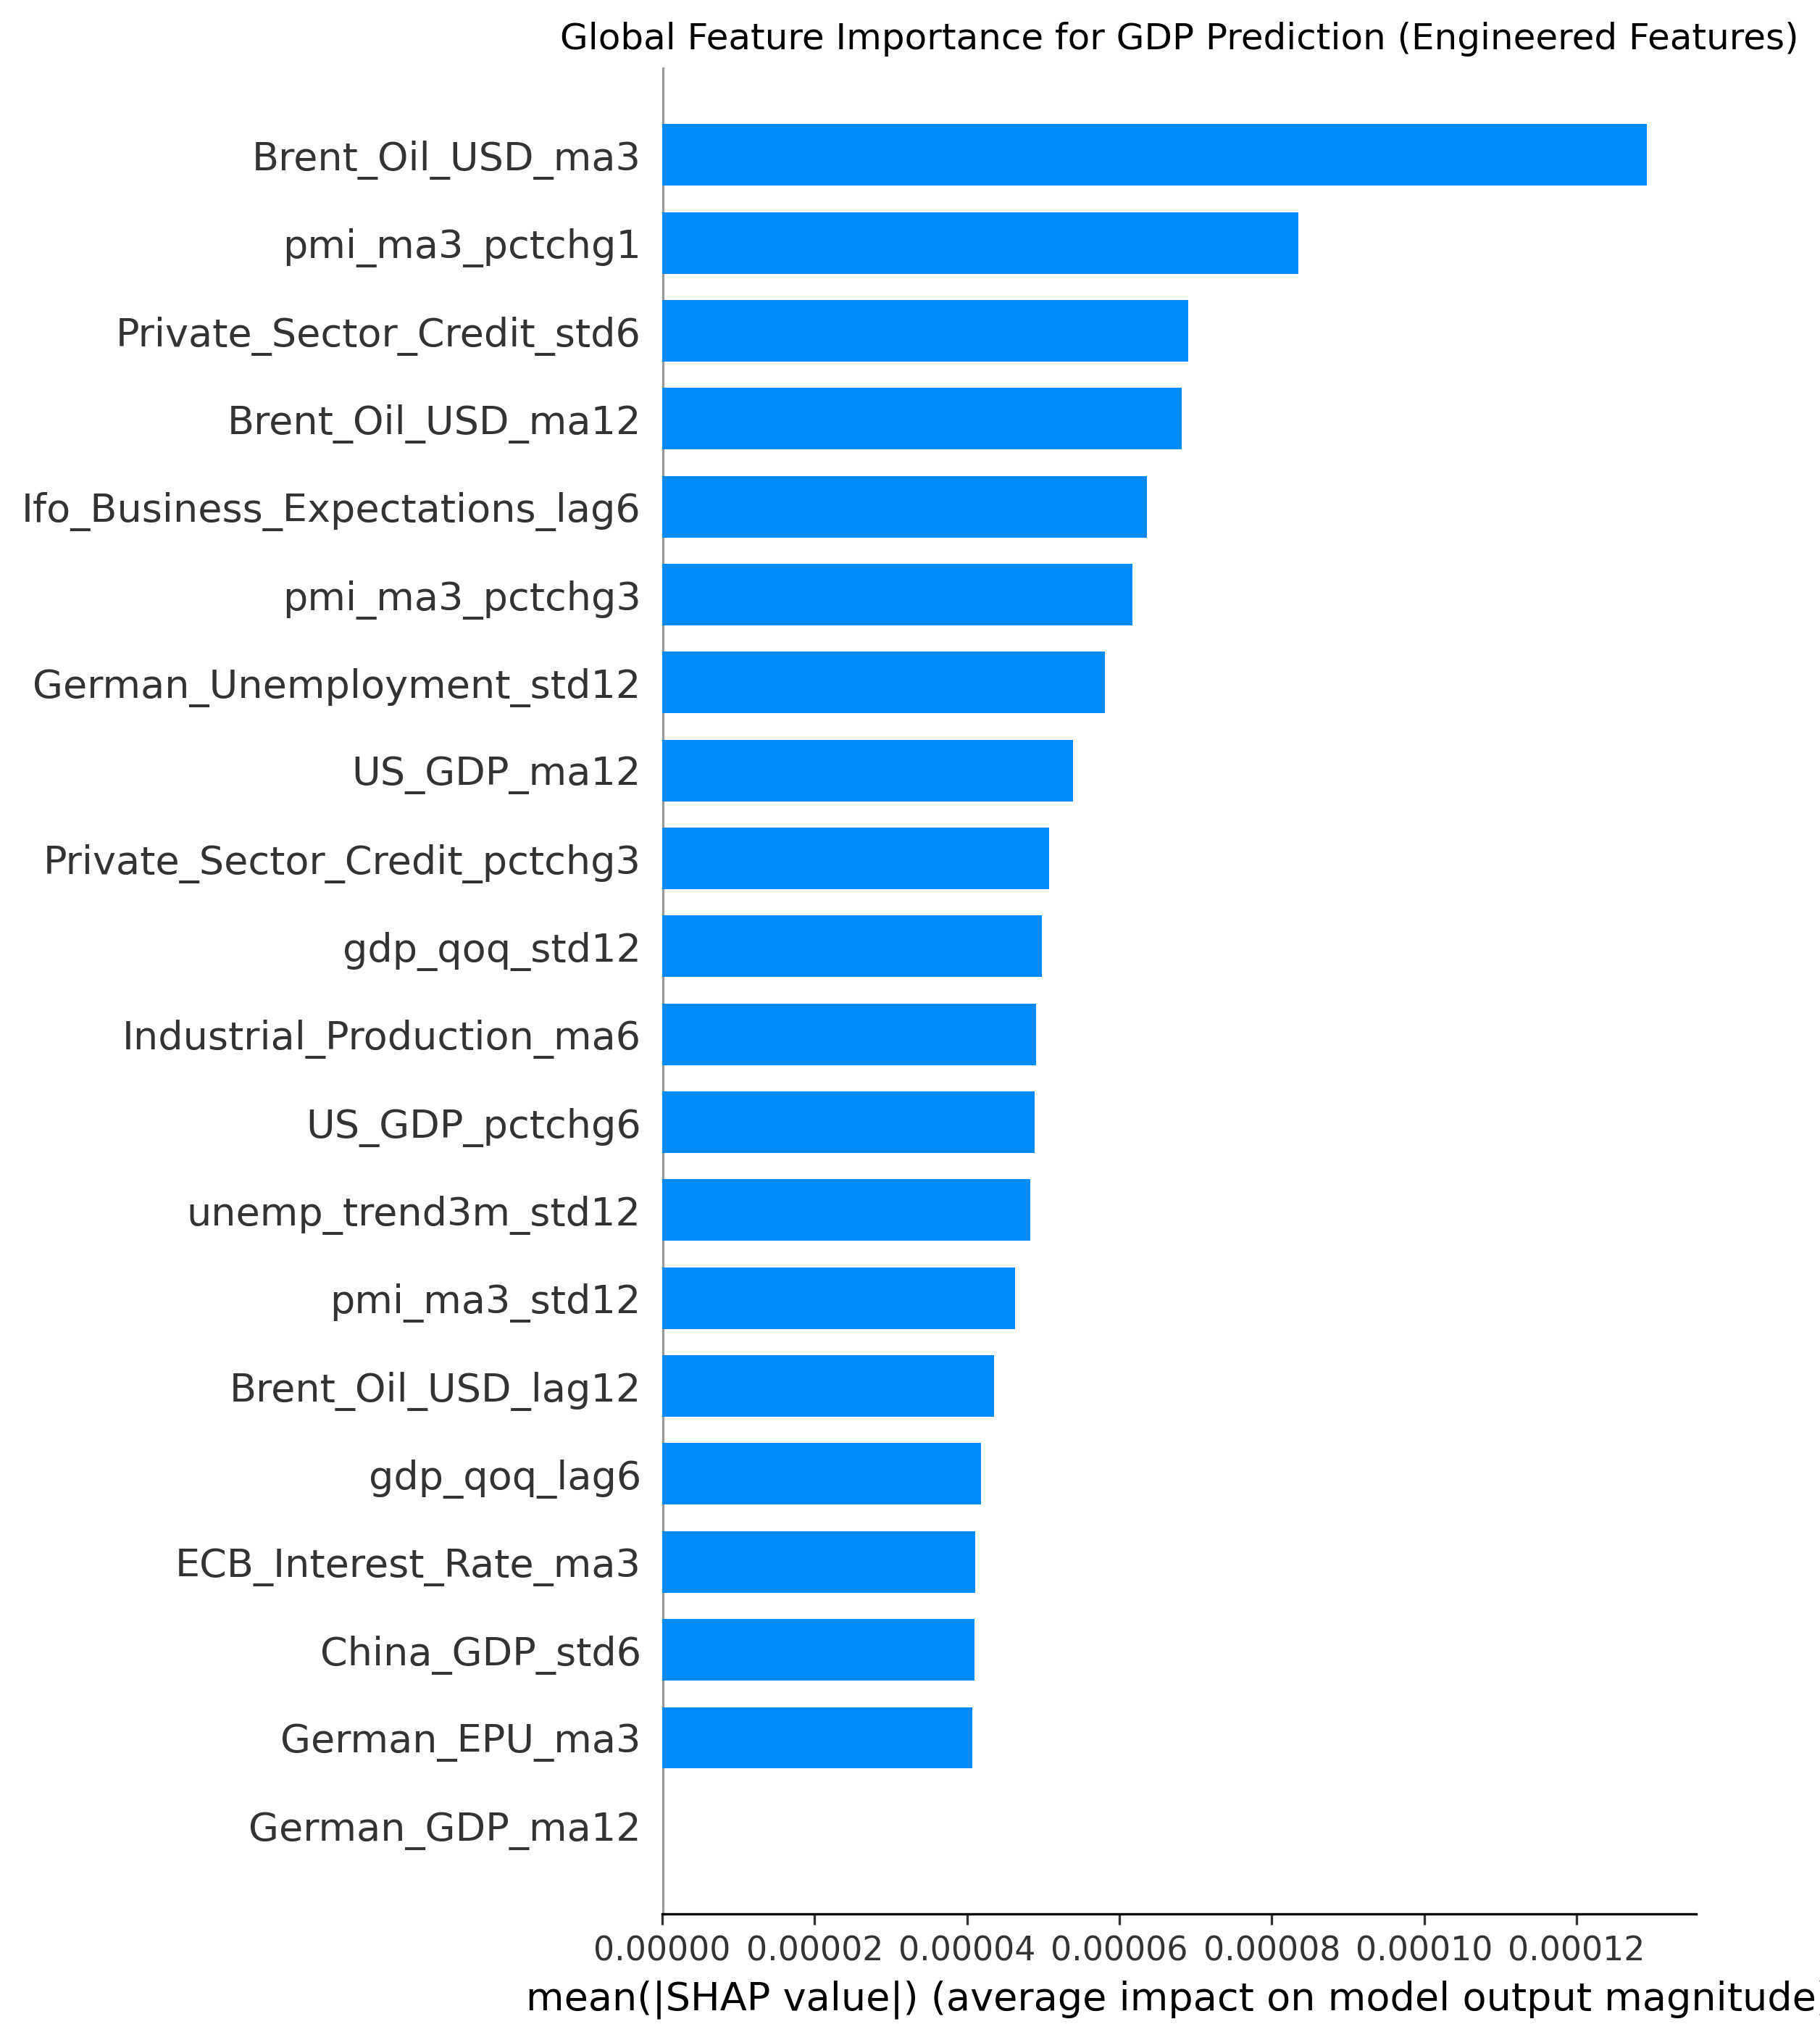
\includegraphics[width=1\textwidth]{images/shap_lstm.png}
    \caption{Feature importance of lstm model}
    \label{fig:featureImportanceOfLSTMModel}
\end{figure}

\begin{figure}[H]
    \centering
    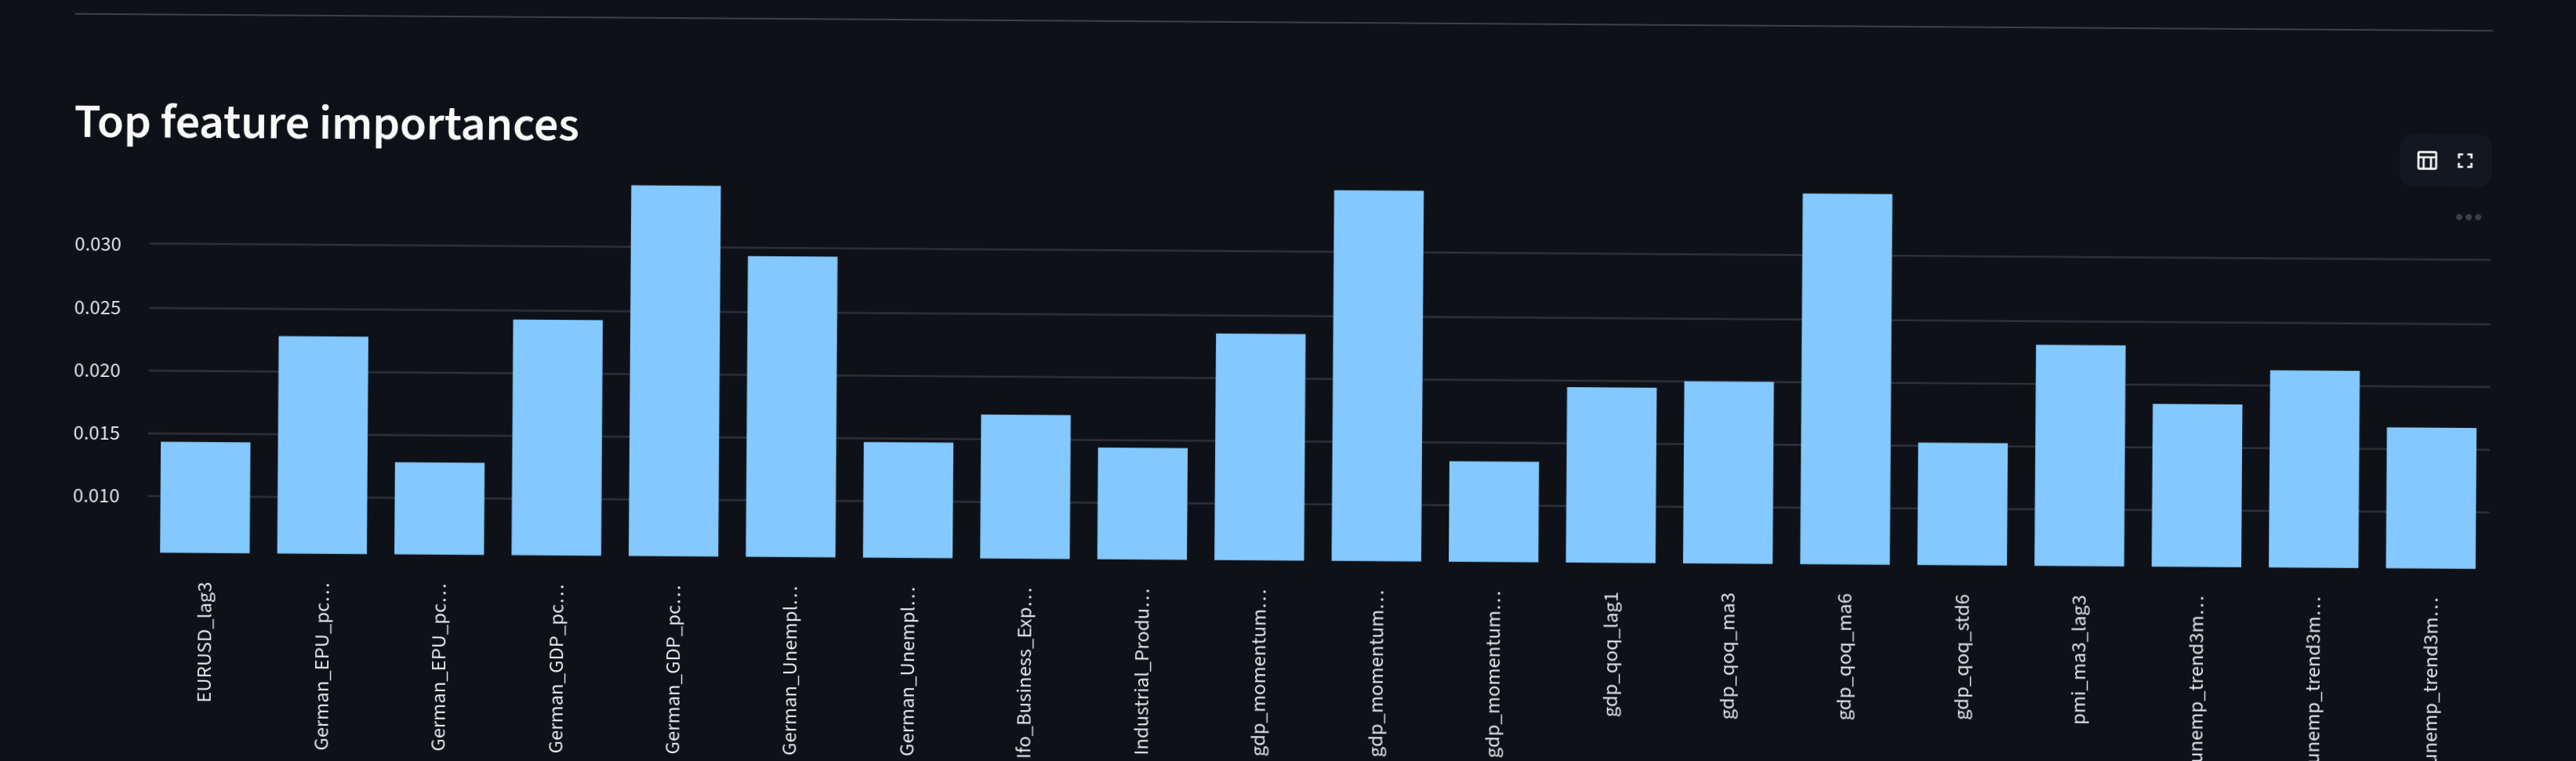
\includegraphics[width=1\textwidth]{images/classification.png}
    \caption{Feature importance of classification model}
    \label{fig:featureImportanceClassification}
\end{figure}

\subsection{Approach}
\label{sec:approach} Two models were selected for two different tasks, LSTM is for predicting gdp growth rate predictions and xgboost for the classification. Starting from the lstm model it became really obvious that lstm has big overfitting, it happened because model had to much units at the beginning it was \textit{64}, thus model didn't find patterns in test data, but rather tried to remember the whole dataset, since it had more than enough capability to remember it and the result of the training might be seen on the figure below. 

\begin{figure}[H]
    \centering
    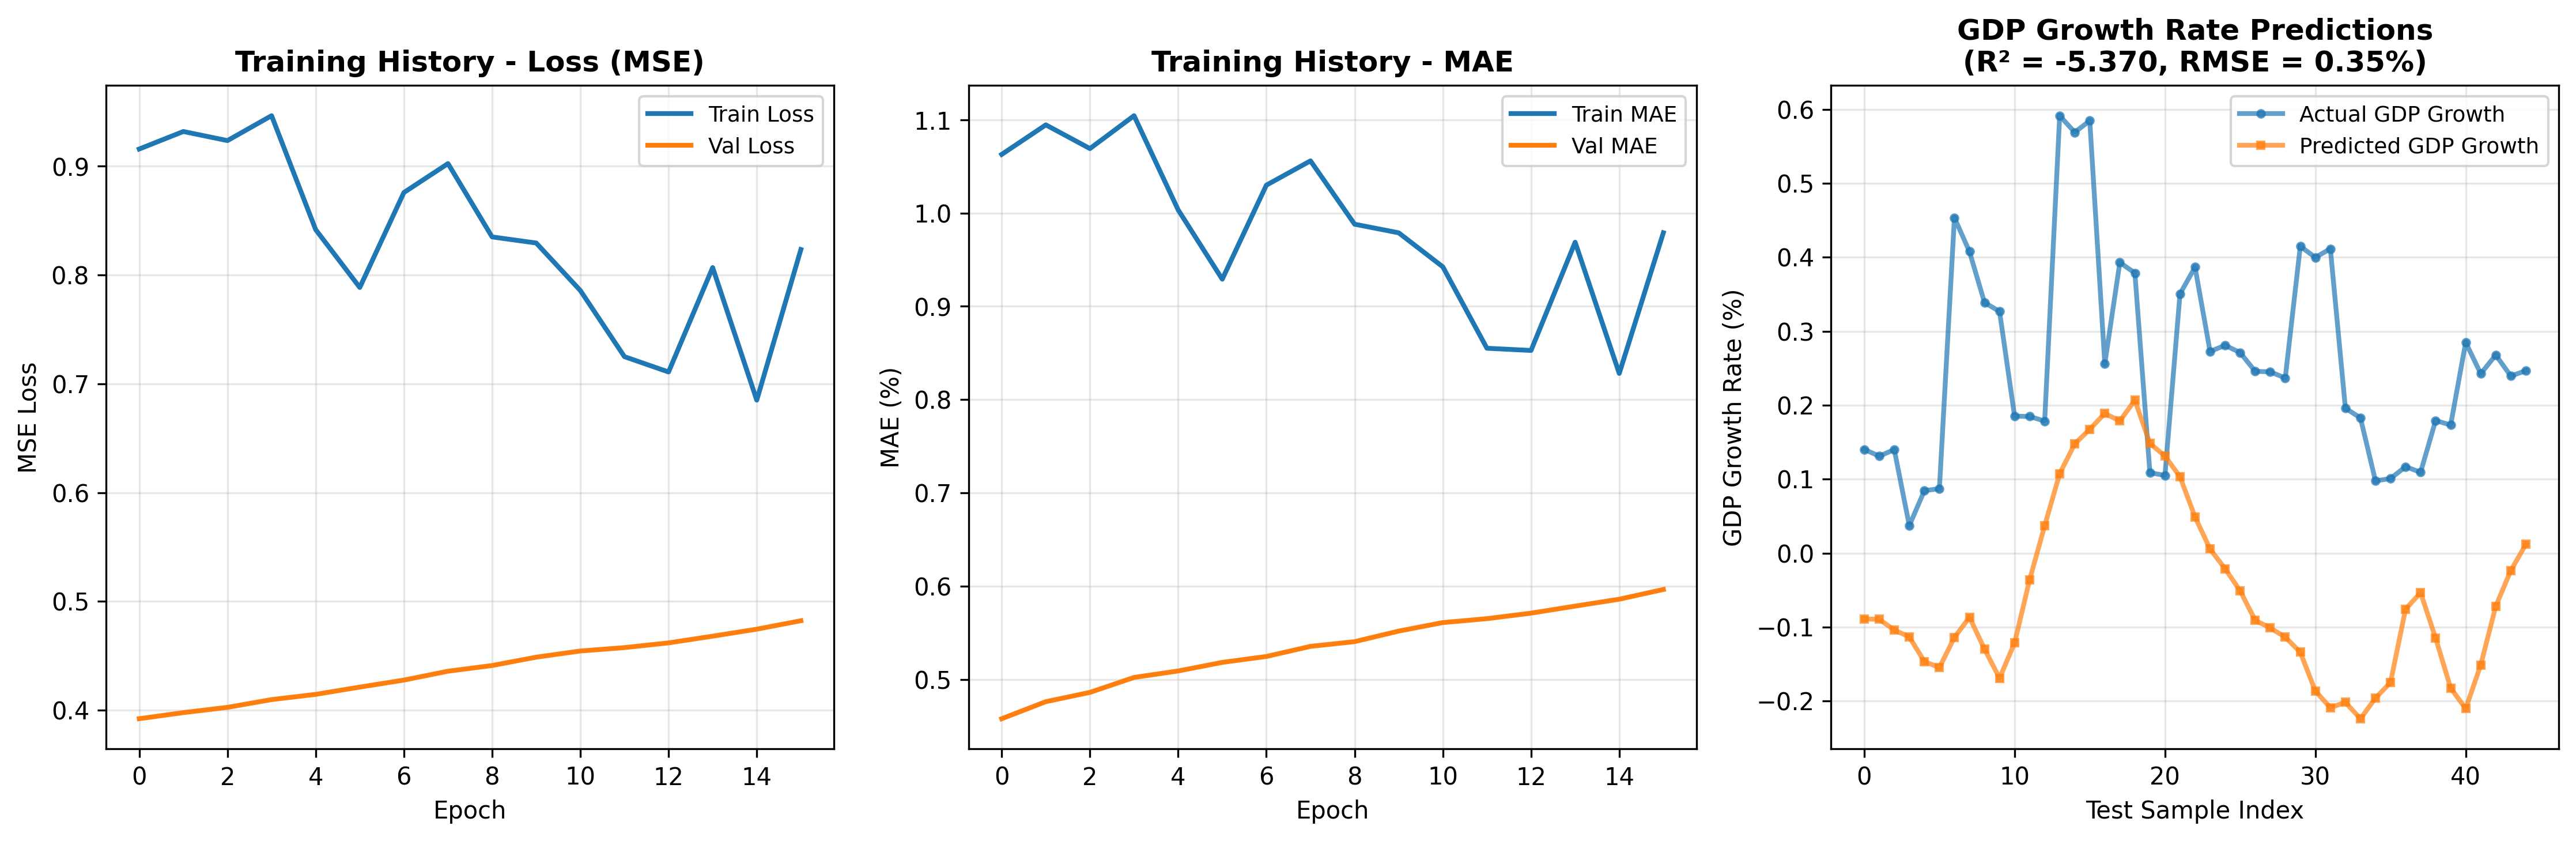
\includegraphics[width=1\textwidth]{images/lstm_training_results.png}
    \caption{LSTM training results}
    \label{fig:lstmTrainingResults}
\end{figure}

Train loss has a momentum down, however it shows negative results, meaning that model doesn't capture underlying patterns, the same picture can be seen on MAE plot. Predictions plot is also does look weak, the best result would have been if predictions overlapped, actual values on the plot, however in the reality it is visible that model instead of predicting highly volatile data, picks strategy of smoothing, the answers.

The reasons above required the change in model behaviour and redefinition of goals, thus the following changes has been applied to the model and data sampling. Goal redefinition now instead predicting growth rate, model predicts only direction gdp will go up or down. Features, amount of features were too overwhelming for model and thus has to be dealt with using \textit{sklearn.decomposition.PCA} amount of features where decreased to 30. Model simplification, simplifying model, model was too complex, now one single lstm layer with 32 units, instead of 3 different layers. Dropout increased, now dropout layers drop almost half of it's incoming signal, making model more focused on underlying patterns. All of the above approaches, resulted in much better picture of model training and evaluation below. 

\begin{figure}[H]
    \centering
    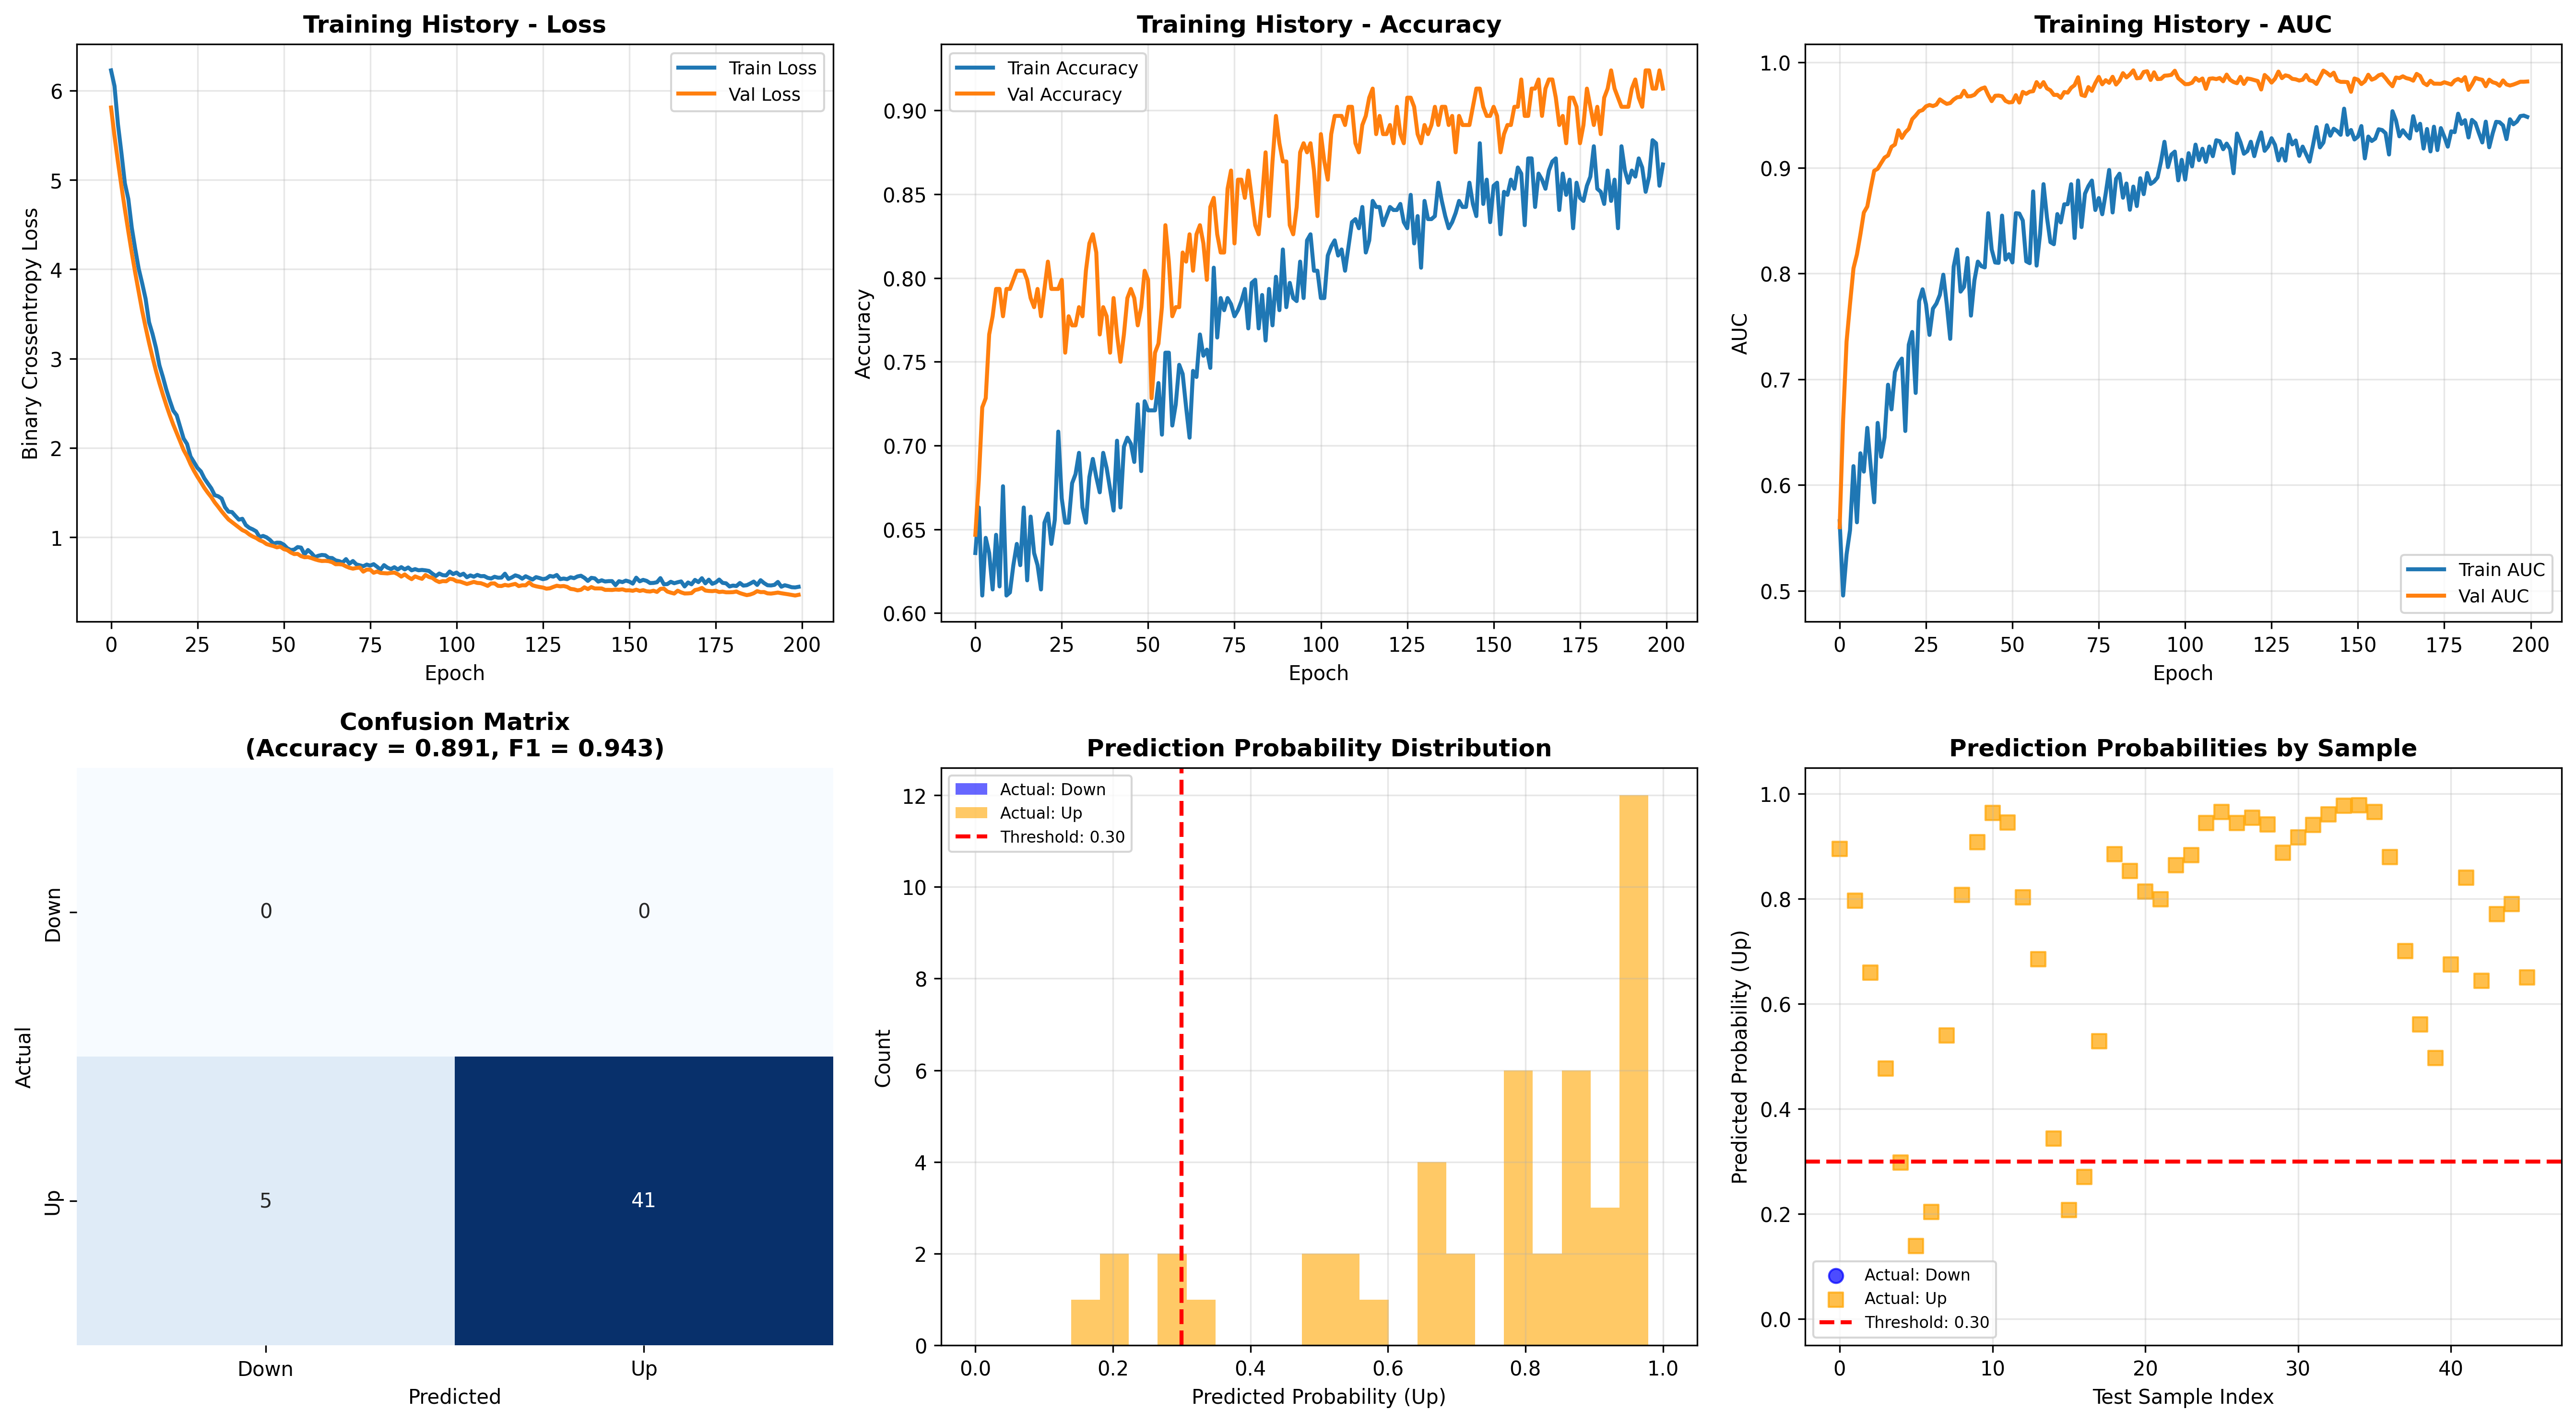
\includegraphics[width=1\textwidth]{images/lstm_training_results_after_goal_change.png}
    \caption{LSTM training results after change}
    \label{fig:lstmTrainingResultsAfterChange}
\end{figure}

One caveat this model has it is that training sample has a very low amount of "down" labels comparing to "up".

On the other hand model which benefited from the big amount of feature is Xgboost, on the evaluation it performed with 96\% accuracy, big part of this was how low population of some classes like \textit{regression} were handled, since sample weights were used it helped to balance a disproportionality of some classes. Dataset classes disproportionality is representation of reality, because in reality \textit{recession} happens rarely.

\begin{figure}[H]
    \centering
    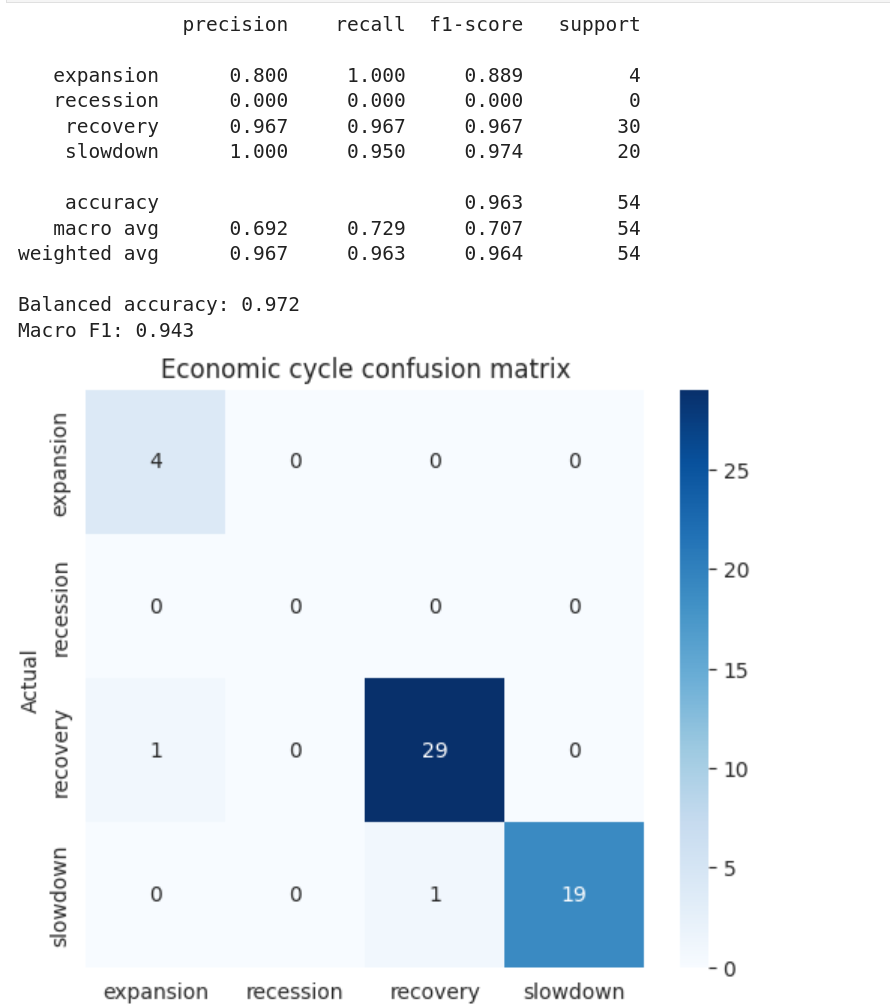
\includegraphics[width=1\textwidth]{images/xgboost_model_results.png}
    \caption{XGBoost training results after change}
    \label{fig:XgboostTrainingResultsAfterChange}
\end{figure}

